\documentclass[a4paper,14pt]{extreport}

% packages to support Cyrillic fonts, needed to write abstracts
\usepackage[T2A]{fontenc} 
\usepackage[utf8]{inputenc} 
\usepackage[russian,english]{babel}
\usepackage{csquotes}
\usepackage{svg}

% usual packages
\usepackage[left=30mm, right=10mm, top=20mm, bottom=20mm]{geometry}

\usepackage{graphicx} % to add figures
\graphicspath{{figures/}}

\usepackage{hyperref} % to add clickable contents menu

\usepackage[style=numeric]{biblatex}
\addbibresource{bibliography.bib}

\usepackage{blindtext}

% the following three definitions are to be changed by student
\def\myauthor{
  Sultan Saliev
  Azamat Rsymbetov
} % author
\def\mycoach{Ualikhan Sadyk} % coach, adviser etc.
\def\mytitle{algomalgo.com - Web Platform for learning Algorithms} % title
\def\mydegree{Bachelor in Computer Science}
\def\mydegreecode{6B06102}

% preamble ends here

\begin{document}
% don't touch these two lines :)
\begin{titlepage}
\begin{center}
\large
Ministry of Education and Science of the Republic of Kazakhstan

Suleyman Demirel University

\vspace{1cm}
\begin{figure}[h]
    \centering
    
\includegraphics[scale=0.5]{sdu_only}
\end{figure}

\vspace{2cm}
\Large
\myauthor

\vspace{1cm}
\Large
\textbf{\mytitle}

\vspace{1cm}
\large
A thesis submitted for the degree of

\mydegree

(degree code: \mydegreecode)

\vfill
Kaskelen, 2020

\end{center}
\end{titlepage}
\newpage
\pagestyle{empty}

\begin{center}
\large
Ministry of Education and Science of the Republic of Kazakhstan

Suleyman Demirel University

Faculty of Engineering and Natural Sciences

\vspace{2cm}
\textbf{\mytitle}

\vspace{1cm}
\large
A thesis submitted for the degree of

\mydegree

(degree code: \mydegreecode)

\vspace{2cm}
Authors: \textbf{\myauthor}

\vspace{2cm}
Supervisor: \textbf{\mycoach}

\vspace{2cm}
Dean of the faculty:

\textbf{Assist. Prof. Andrey Bogdanchikov}


\vfill
Kaskelen, 2020
\end{center}

% edit abstracts
\newpage
\pagestyle{plain}

\begin{center}
    \Large
    \textbf{Abstract}
\end{center}
This thesis discusses the gamification or use of game elements in non-game contexts, as well as its potential use in education to enhance student motivation and involvement. The use of technology helps to increase the effectiveness of training. Mobile devices are designed to be powerful mini-computers, and the potential for learning on these devices is growing. This means that people can learn using interactive technology whenever and wherever they wish using their own personal devices. You can add different elements of gamification to different types of training. In the future, it will be possible to integrate this method into state institutions, such as schools and universities.
\newpage
\pagestyle{plain}

{\selectlanguage{russian}
\begin{center}
    \Large
    \textbf{Аңдатпа}
\end{center}
Диссертациялық жұмыста ойын элементтерін ойынға қосу немесе қолдану, сондай-ақ оқушылардың ынтасы мен белсенділігін арттыру үшін оны білім беруде қолдану мүмкіндігі қарастырылады. Технологияны қолдану оқытудың тиімділігін арттыруға көмектеседі. Мобильді құрылғылар қуатты мини-компьютерлерге арналған, сондықтан бұл құрылғыларда білім алу мүмкіндігі артып келеді. Бұл дегеніміз, адамдар интерактивті технологияны пайдалана отырып, жеке құрылғыларды қашан және қай жерде қолданғысы келетіндігін біле алады. Әр түрлі жаттығуларға геймификацияның әр түрлі элементтерін қосуға болады. Болашақта бұл әдісті мемлекеттік мекемелерге, мысалы мектептер мен университеттерге біріктіруге болады.
}
\newpage
\pagestyle{plain}

{\selectlanguage{russian}
\begin{center}
    \Large
    \textbf{Аннотация}
\end{center}
В этом тезисе обсуждается геймификация или использование игровых элементов в неигровых контекстах, а также ее потенциальное применение в образовании для усиления мотивации и вовлеченности учащихся. Использование технологий способствует повышению эффективности обучения. Мобильные устройства разрабатываются для того, чтобы они были мощными мини-компьютерами, и потенциал для обучения на этих устройствах становится все больше. Это означает, что люди могут учиться, используя интерактивные технологии, когда и где они пожелают, используя свои собственные персональные устройства. Можно добавить различные элементы геймификации  в различные типы обучения. В дальнейшем можно будет интегрирывать этот метод в государственные учереждения, такие как школы и вузы.
}
\tableofcontents

% edit your chapters
\chapter{Introduction}\label{ch:intro}
%these sections are optional, up-to the author
\section{Motivation}
Informally, an algorithm is any well-defined computational procedure that takes some value, or set of values, as input and produces some value, or set of values, as output. An algorithm is thus a sequence of computational steps that transform the input into the output.
We can also view an algorithm as a tool for solving a well-specified computational problem. The statement of the problem specifies in general terms the desired input/output relationship. The algorithm describes a specific computational procedure for achieving that input/output relationship. \\
                    
For example, we might need to sort a sequence of numbers into nondecreasing order. This problem arises frequently in practice and provides fertile ground for introducing many standard design techniques and analysis tools. Here is how we formally define the sorting problem: \\

Input: $\langle a_1, a_2, a_3 ... a_n \rangle$

Output: A permutation (reordering) $\langle a^{'}_1, a^{'}_2, a^{'}_3 ... a^{'}_n \rangle$ \\

For example, given the input sequence $\langle 31, 41, 59, 26, 41, 58 \rangle$ a sorting algorithm returns as output the sequence $\langle 26, 31, 41, 41, 58, 59 \rangle$. Such an input sequence is called an instance of the sorting problem. In general, an instance of a problem consists of the input (satisfying whatever constraints are imposed in the problem statement) needed to compute a solution to the problem. \\

In the present age, people who aspire to work in those fields learn frameworks and libraries that abstract away the use of algorithms and hide the computational cost of each used function. Generally, that is a good thing, because it greatly improves their workflow and makes those professions more accessible, thus reducing the costs of production. However, the downsides are that it affects the software quality, decreasing performance and using large amounts of memory. One of the recent examples of algorithm misuse that appeared globally is a GTA V game, where the if statement was triggered 1.98 billion times while preloading the GTA V online screen.

As you can see, algorithms are the basis of all computational problems, thus it could be seen as an essential tool for everyone in the computer science field including: software engineers, computer science researchers, data scientists, machine learning engineers, data engineers, etc.


\section{Aims and Objectives}
Our project is aimed to make a decent contribution to educating people who aspire to enter career in Computer Science related professions.

\section{Thesis Outline}
The first chapter is an \textit{\nameref{ch:intro}} chapter. This chapter introduces you to gamification and describes aims of this thesis. The second chapter is \textit{\nameref{ch:1}}, which describes the gaming industry. Since it is important to find out why people like to play games, and how to direct this interest in the right direction. Chapter three is the \textit{\nameref{ch:3}}, which explains about implementation experience and basic gamification techniques. In chapter \textit{\nameref{ch:4}} observations and comparisons of gamification material are described.

\chapter{The Origin of Algorithms}\label{ch:1hkdh,kxch,.kdh,}
\section{Matematician from Uzbekistan}

\begin{figure}[h]
    \centering
    
\includegraphics[scale=0.4]{figures/alkhwarizmi.png}
    \caption{Abu Abdullah Muhammad ibn Musa Al-Khawarizmi}
    \label{fig:gp}
\end{figure}

The term algorithm got its name from the Persian astronomer and mathematician, Abu Abdullah Muhammad ibn Musa Al-Khawarizmi (780 AD).\\
He was from a Persian city known as Khwarizm, found in present-day Uzbekistan.\\
Al-Khwarizmi wrote many important mathematical books that were later translated into Latin.\\
It was his book on Arabic-Hindu numerals and arithmetic, called Al-Khw?rizm? On the Hindu Art of Reckoning, later Latinized as Algoritmi de numero Indorum that gave the word algorithm to the Western world. \\

\pagebreak

\section{First Algorithm}

\begin{figure}[h]
    \centering
    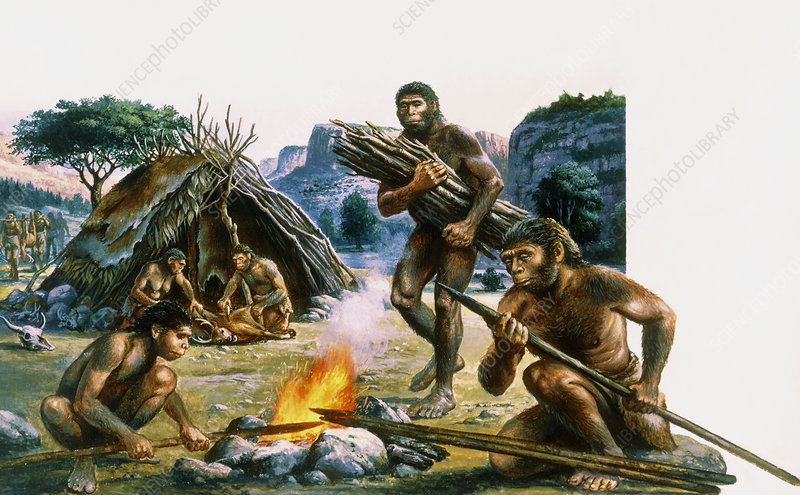
\includegraphics[scale=0.4]{figures/homo_erectus.jpg}
    \caption{Homo Erectus}
    \label{fig:gp}
\end{figure}

Generally, the existence of algorithms as long as human history. As an example, the creation of the first artificial fire in the Wonderwerk Cave of South Africa, millions of years ago by Homo Erectus, constitutes our first evidence of the use of algorithms. However, most historians hold the view that the Babylonian clay tablets (1600-1800 BC) are the world's first known algorithm. The Babylonians had developed a numerical system using cuneiform numerals to count and they preserved those calculations on tablets. \\ 

\begin{figure}[h]
    \centering
    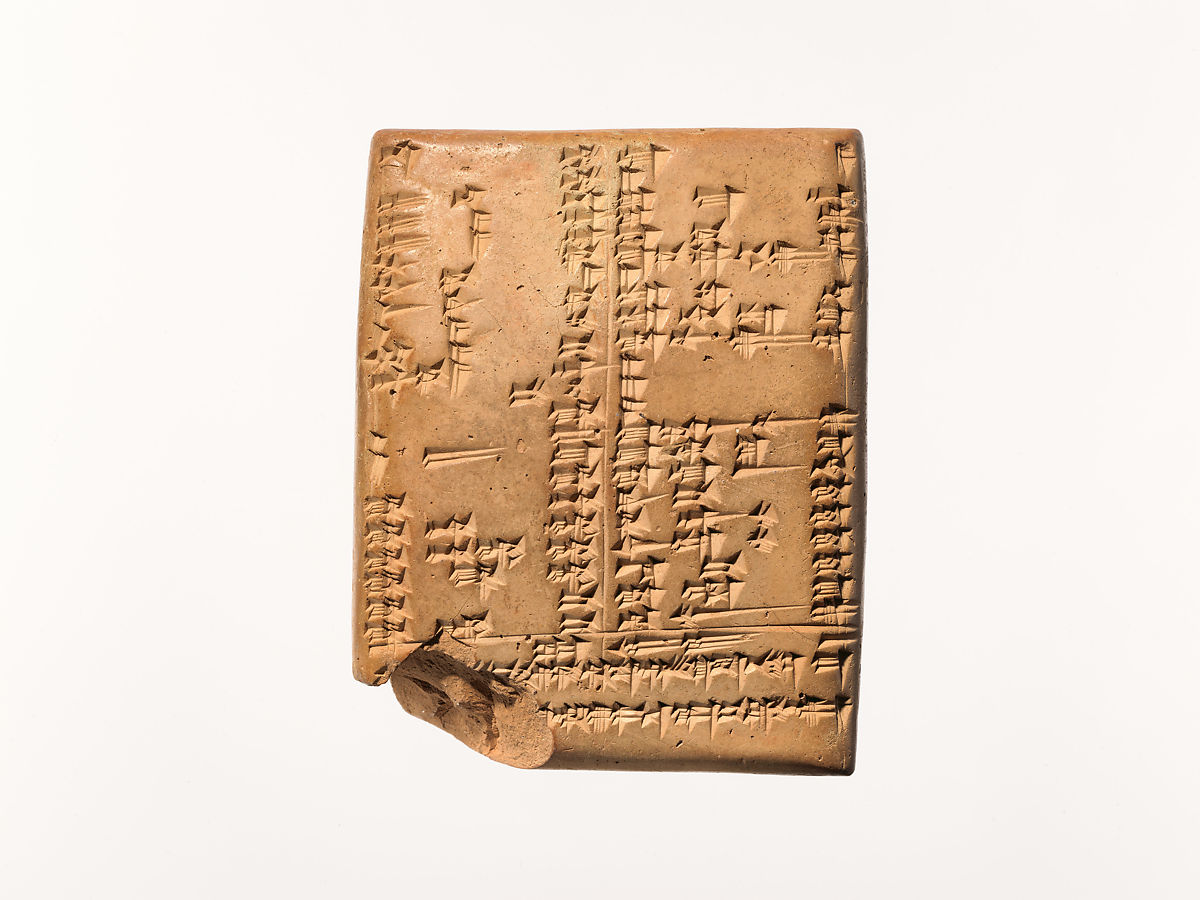
\includegraphics{figures/tablet.jpg}
    \caption{Cuneiform tablet}
    \label{fig:gp}
\end{figure}

Although we can find instances of algorithms in Euclidean mathematics,\\
Archimedes approximation of Pi, or Eratosthenes calculation of prime numbers, it was the work of George Boole in developing what is known as Boolean algebra, in 1847, that set the basis for computer logic today. Boole developed a system of logic to make calculations that used true and false values as basic units (binary algebra). This system would later be represented in digital form by zeros and ones or binary digits in low-level programming languages. \\ 

\section{Computing machine}

Some decades later, Alan Turing came up with a mathematical model of a hypothetical computing machine. It used squares that contained symbols or binary digits in an infinitely long tape. This tape served as storage space for the data in the squares, computer memory. It has a head or needle that can move to the right or left of each square to read, write, or erase the symbol within it, the basis for CRUD (Create, Read, Update, and Delete) operations in programming. Using this system this machine could simulate any algorithm, regardless of its complexity!
Mathematicians and computer scientists continued adding to Turing's concept of a computing machine to advance technology to what we know today. Algorithms then evolved from binary operations to high-level, more human-friendly, programming languages like C++, Java, and etc. Because they allow creating efficient, error-free software applications, they will continue to be important in the foreseeable future. \\ 


\begin{figure}[h]
    \centering
    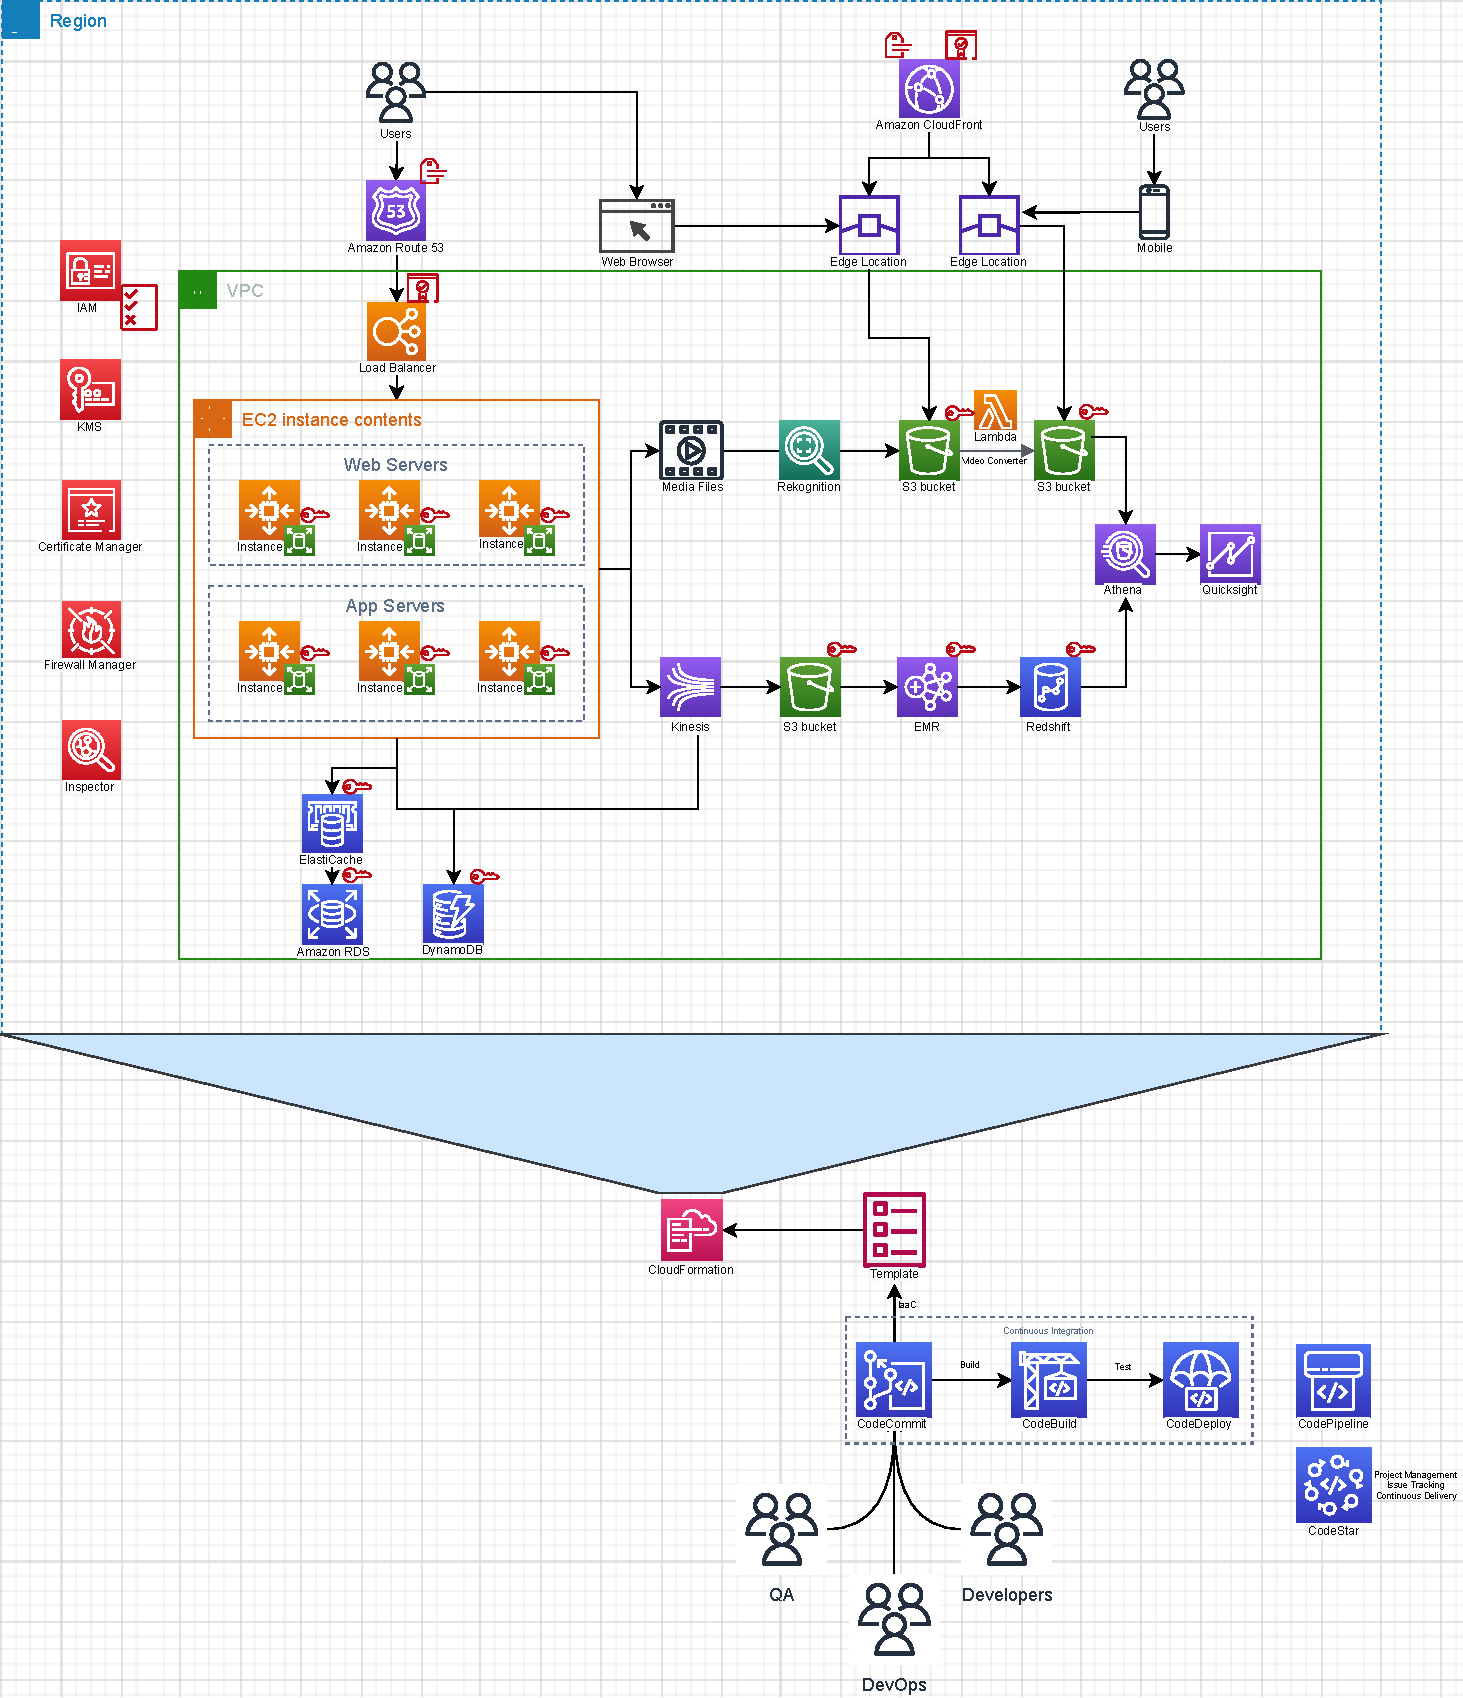
\includegraphics[scale=0.7]{figures/sys.pdf}
    \caption{System Design}
    \label{fig:gp}
\end{figure}

\chapter{The Death of Moore’s Law}\label{ch:3}
\section{Introduction}

The advent of RISC computing in the 1980s was the basis for Gordon Moore's initial prediction and faithfully showed a doubling in processor performance every 18 months. But, as the limits of clock frequency per chip began to appear, the use of Dennard scaling and multicore CPUs helped prolong the performance curve. But it is important to note that even at the start of the century, we were no longer on the Moore's Law curve, and doubling of performance took 3.5 years during this time. \\

Amdahl's Law refers to the limits of performance improvement that can be achieved with parallel processing. While parallelizing the execution of a process can provide an initial performance boost, there will always be a natural limit, as there are some execution tasks that cannot be parallelized. We have recently experienced that these limits come into effect when the benefits of using multiple CPU cores decrease, leading to an even longer time span between performance improvements. \\
The prediction, as can be seen in the graph, is that it will now take 20 years for CPU processing power to double in performance. Hence, Moore's Law is dead. \\

\pagebreak

\begin{figure}[h]
    \centering
    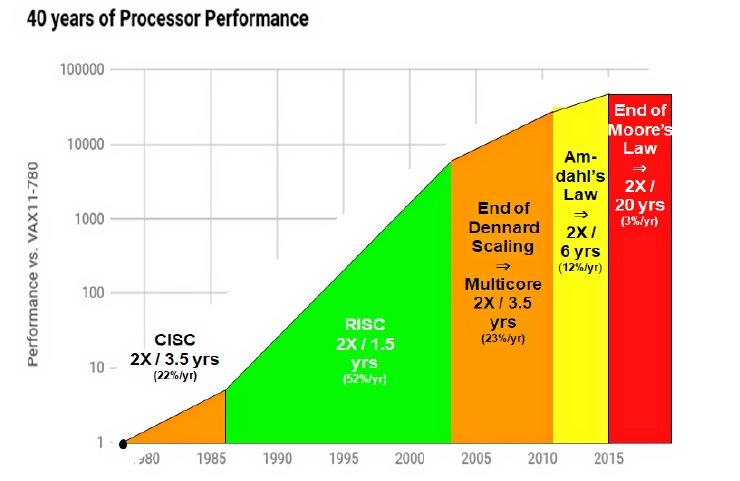
\includegraphics[scale=0.7]{figures/processor-performance.png}
    \caption{Source: John Hennessy and David Patterson, Computer Architecture: A Quantitative Approach, 6/e. 2018}
    \label{fig:gp}
\end{figure}

However, the underlying business model assumption here is that as the number of clients and volume of work increases, it is enough to simply add more servers. But, as can be clearly seen in the earlier graph, server processing performance will only grow 3\% per year over the next 20 years. This is far below the expectation that the amount of data to be processed will triple over the next five years
That's why the efficient use of that hardware is more important than ever and that requires the knowledge of algorithms and data structures. \\

\section{Algorithms in Big Tech Companies}
Most of the companies as a basis of their success used advanced algorithms to scale their service. One of the popular examples is Google, which used advanced web crawler technology and web site indexing to find information across the web. Google’s web crawler algorithm works in such a way, where it explores new sites existing on the web, based on visiting pre-existing site’s links, analyzing over 40,000 new pages in the web per second. After a page is crawled, Google tries to understand what the page is about. This stage is called indexing and it includes processing and analyzing the textual content and key content tags and attributes, such as <title> elements and alt attributes, images, videos, and more. All the process could be seen as a graph traversal procedure, where its page could be seen as a single node and links between pages could be viewed as edges. Using these technologies, they became a one of the significal companies in their field. \\

Another decent example could be Alibaba group, which used advanced algorithms in their cloud computing service in order to perform well on Single’s day, when the number of orders were at its peak. During this day Alibaba cloud processed 175,000 transactions and 120,000 per second at peak traffic, earning for a company around 84.54 billion U.S. dollars for two weeks according to 2021 yearly report. In order to perform well, they have used the Apache Flink framework, to distribute real time data across many clusters. However, to divide that data into meaningful chunks, they have used a sliding window algorithm, which is one of the most popular algorithms. Thus, the knowledge of good algorithms helped them to achieve their goal. \\

\begin{figure}[h]
    \centering
    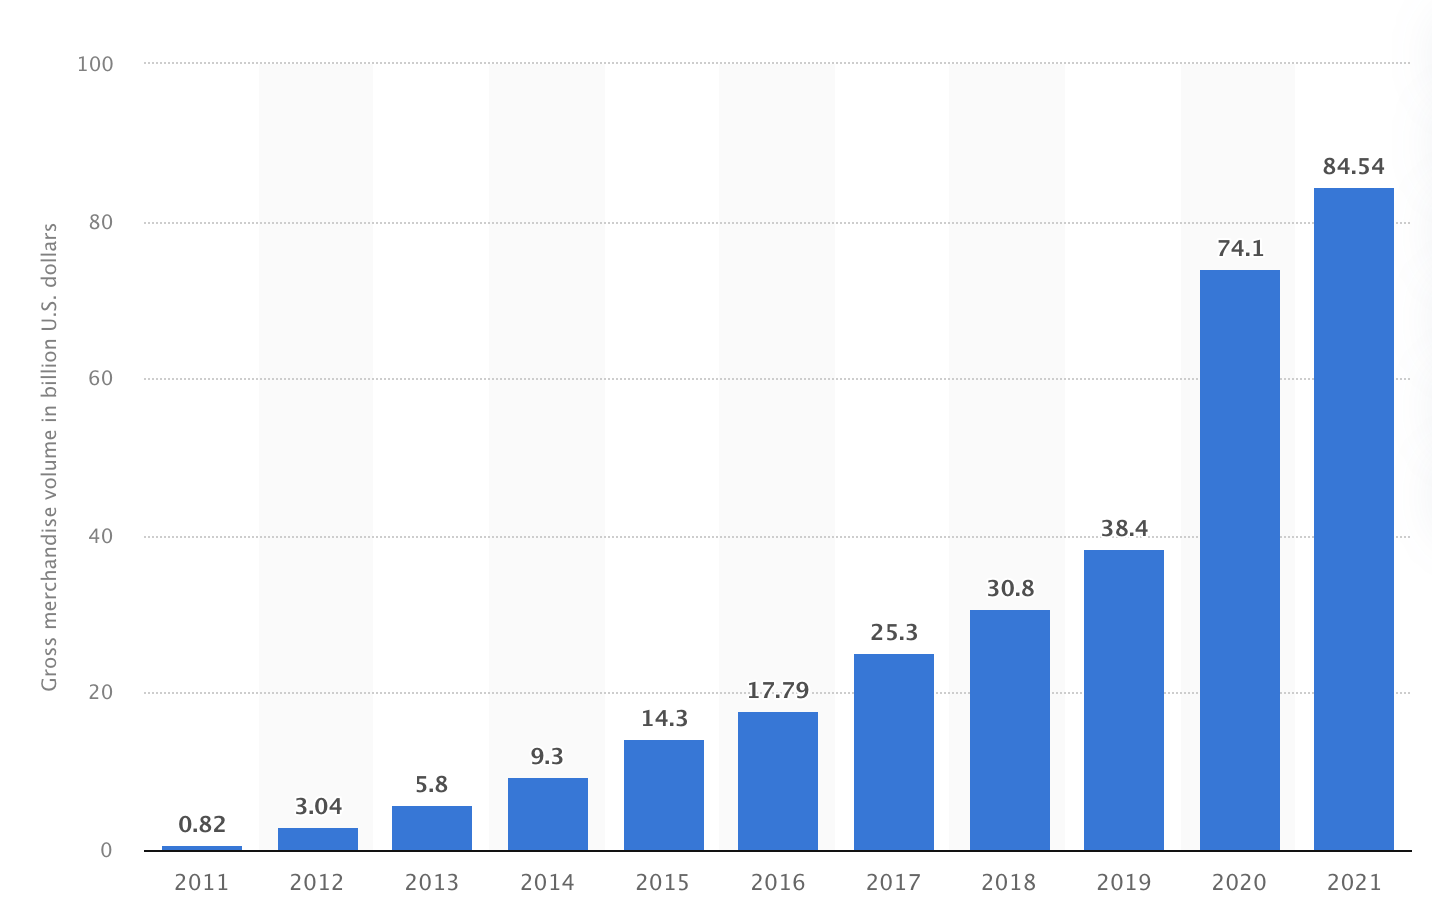
\includegraphics[scale=0.6]{figures/alibaba.png}
    \caption{Alibaba's gross merchandise volume on Singles' Day from 2011 to 2021 (in billion U.S. dollars)}
    \label{fig:gp}
\end{figure}

The other example could be Amazon, which incrementally updated the quality of their services in order to perform well on the market. At first, they only had e-commerce website with some goods, however to increase interest rate, they started to invent various algorithms, one of the examples is collaborative filtering algorithm, which was revolutionary 20 years ago. After a few years they have improved their algorithm adding some heuristics and by increasing computational power they made items on their site more customizable for a specific person, which greatly boosted the amount of their revenue in Amazon, Amazon Kindle and Amazon Prime. As for today, they use multilayered collaborative neural networks, to make the best possible predictions, which will be beneficial for their business.\\

Uber could be another good example, they use sophisticated path finding algorithms as Dijkstra and A star for cost and time optimization purposes. Using these algorithms at their core, they have created a good customer experience, which led to its becoming a multi-billion company.

\input{chapterC}
\chapter{Implementation}\label{ch:5}
\subsection{Tech Stack}

\begin{figure}[h]
    \centering
    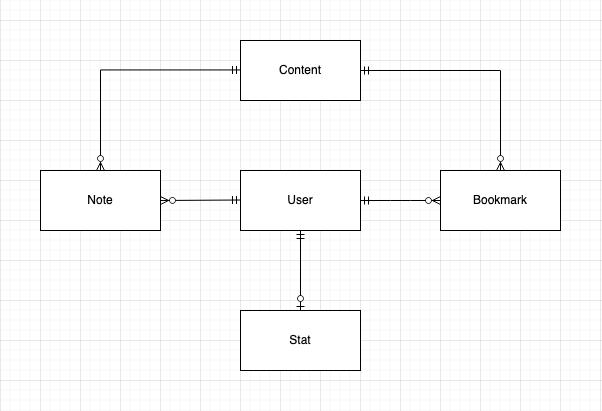
\includegraphics[scale=0.5]{figures/erd.png}
    \caption{Entity Relationship Diagram}
    \label{fig:gp}
\end{figure}

\pagebreak
Frontend: React.js, Tailwind.css, Next.js \\
Backend: Next.js \\
Database: PostgreSQL \\


\subsection{Wireframes}

\begin{figure}[h]
    \centering
    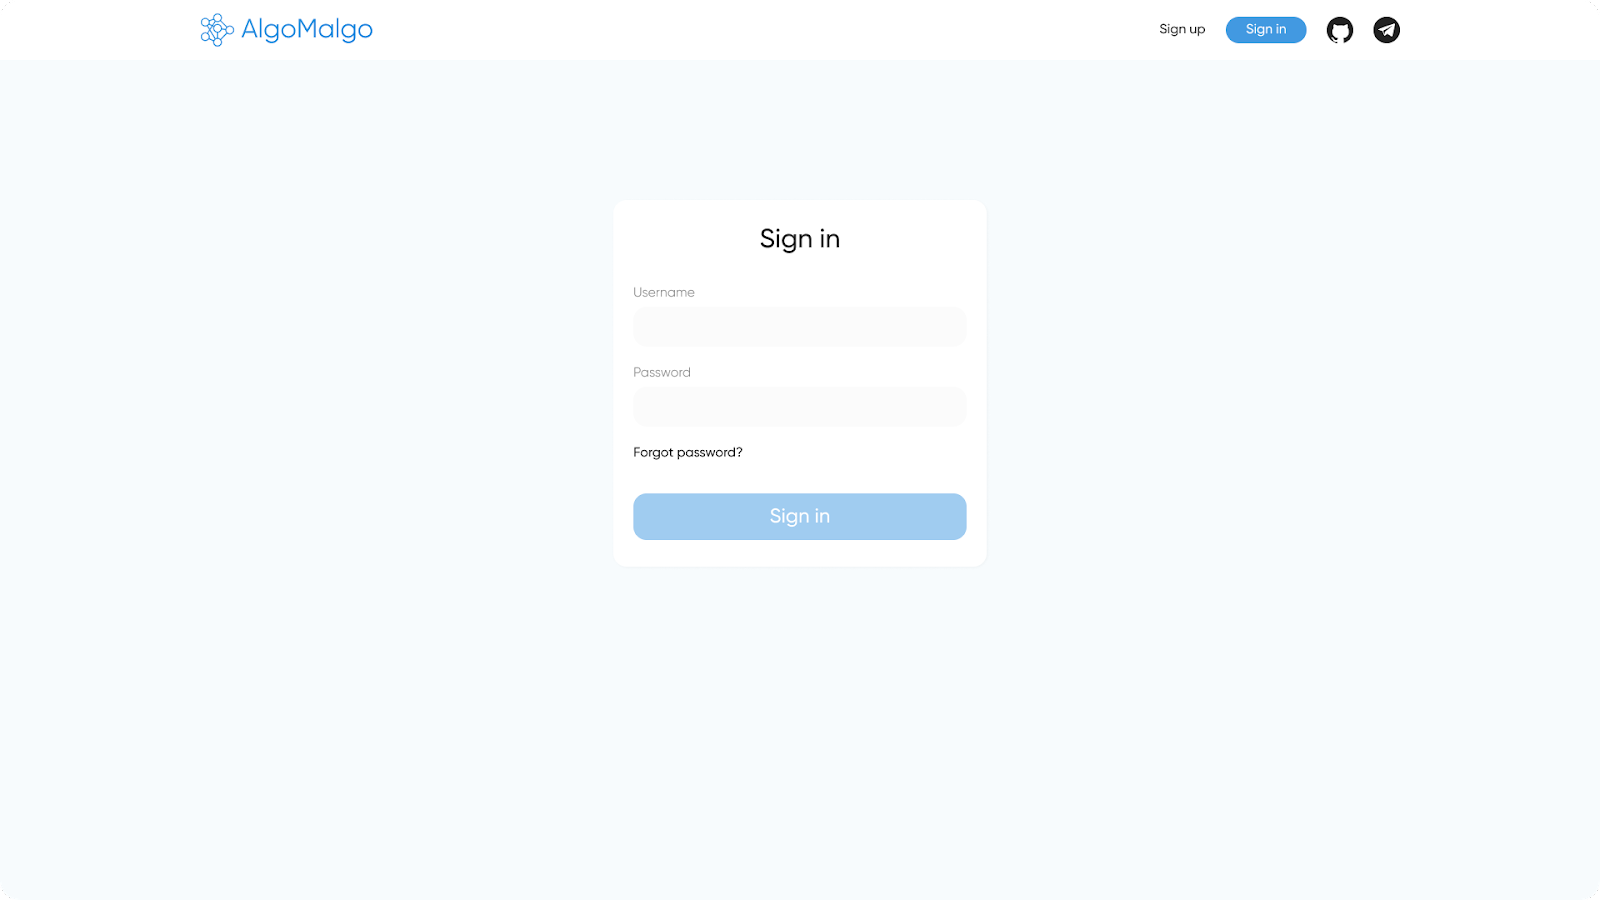
\includegraphics[scale=0.3]{figures/signin.png}
    \caption{Sign In}
    \label{fig:gp}
\end{figure}

\pagebreak

\begin{figure}[h]
    \centering
    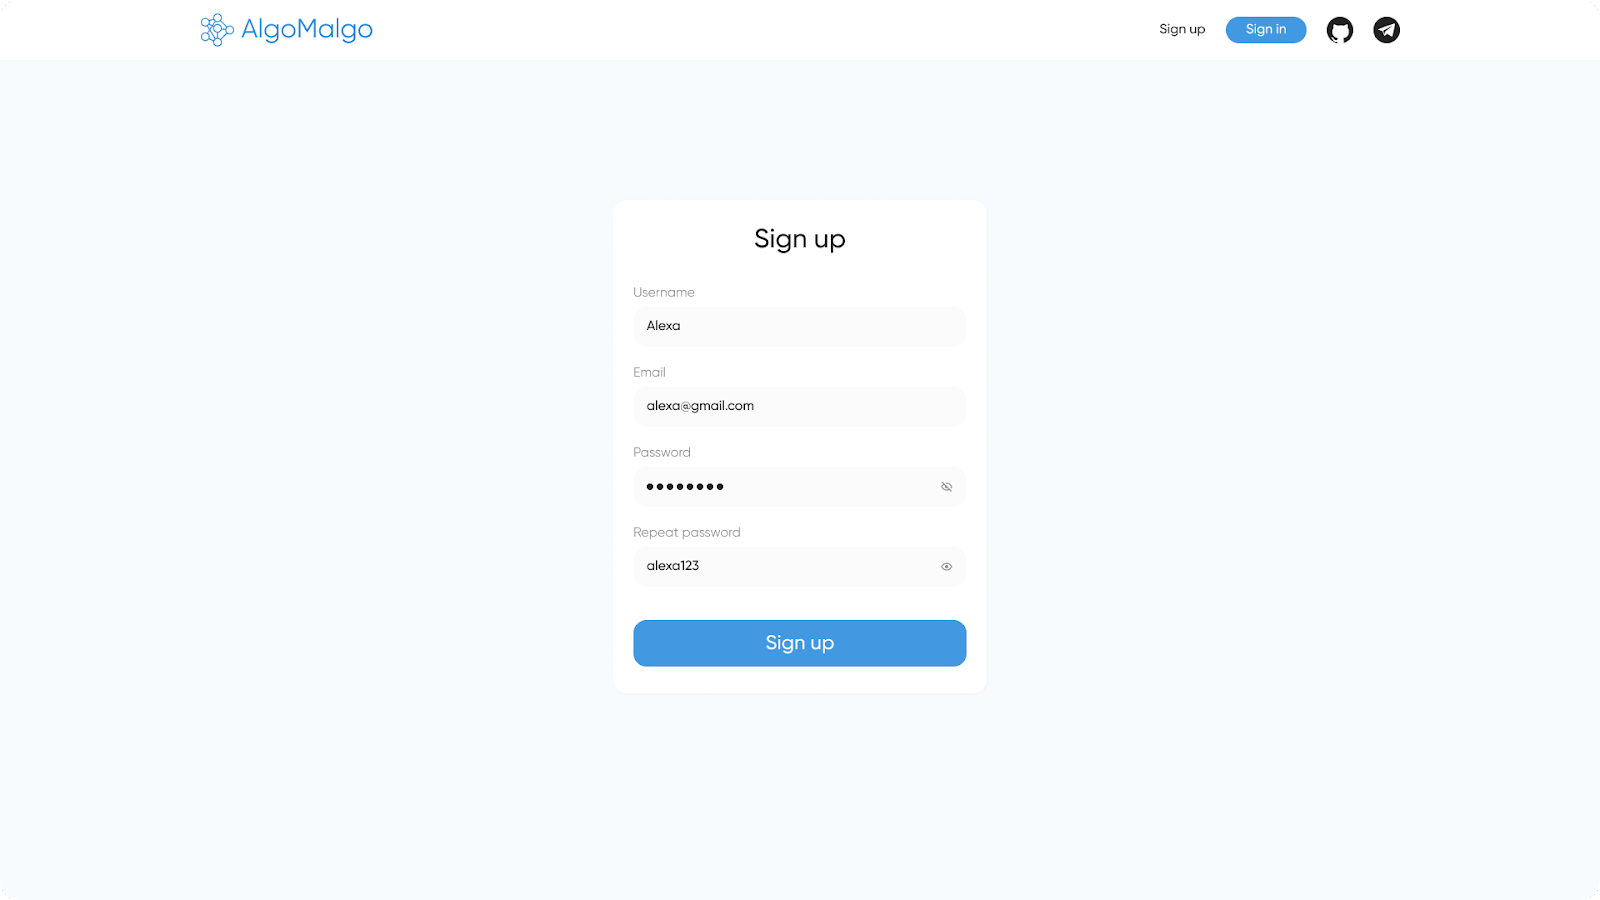
\includegraphics[scale=0.3]{figures/registration.png}
    \caption{Registration}
    \label{fig:gp}
\end{figure}

\pagebreak

\begin{figure}[h]
    \centering
    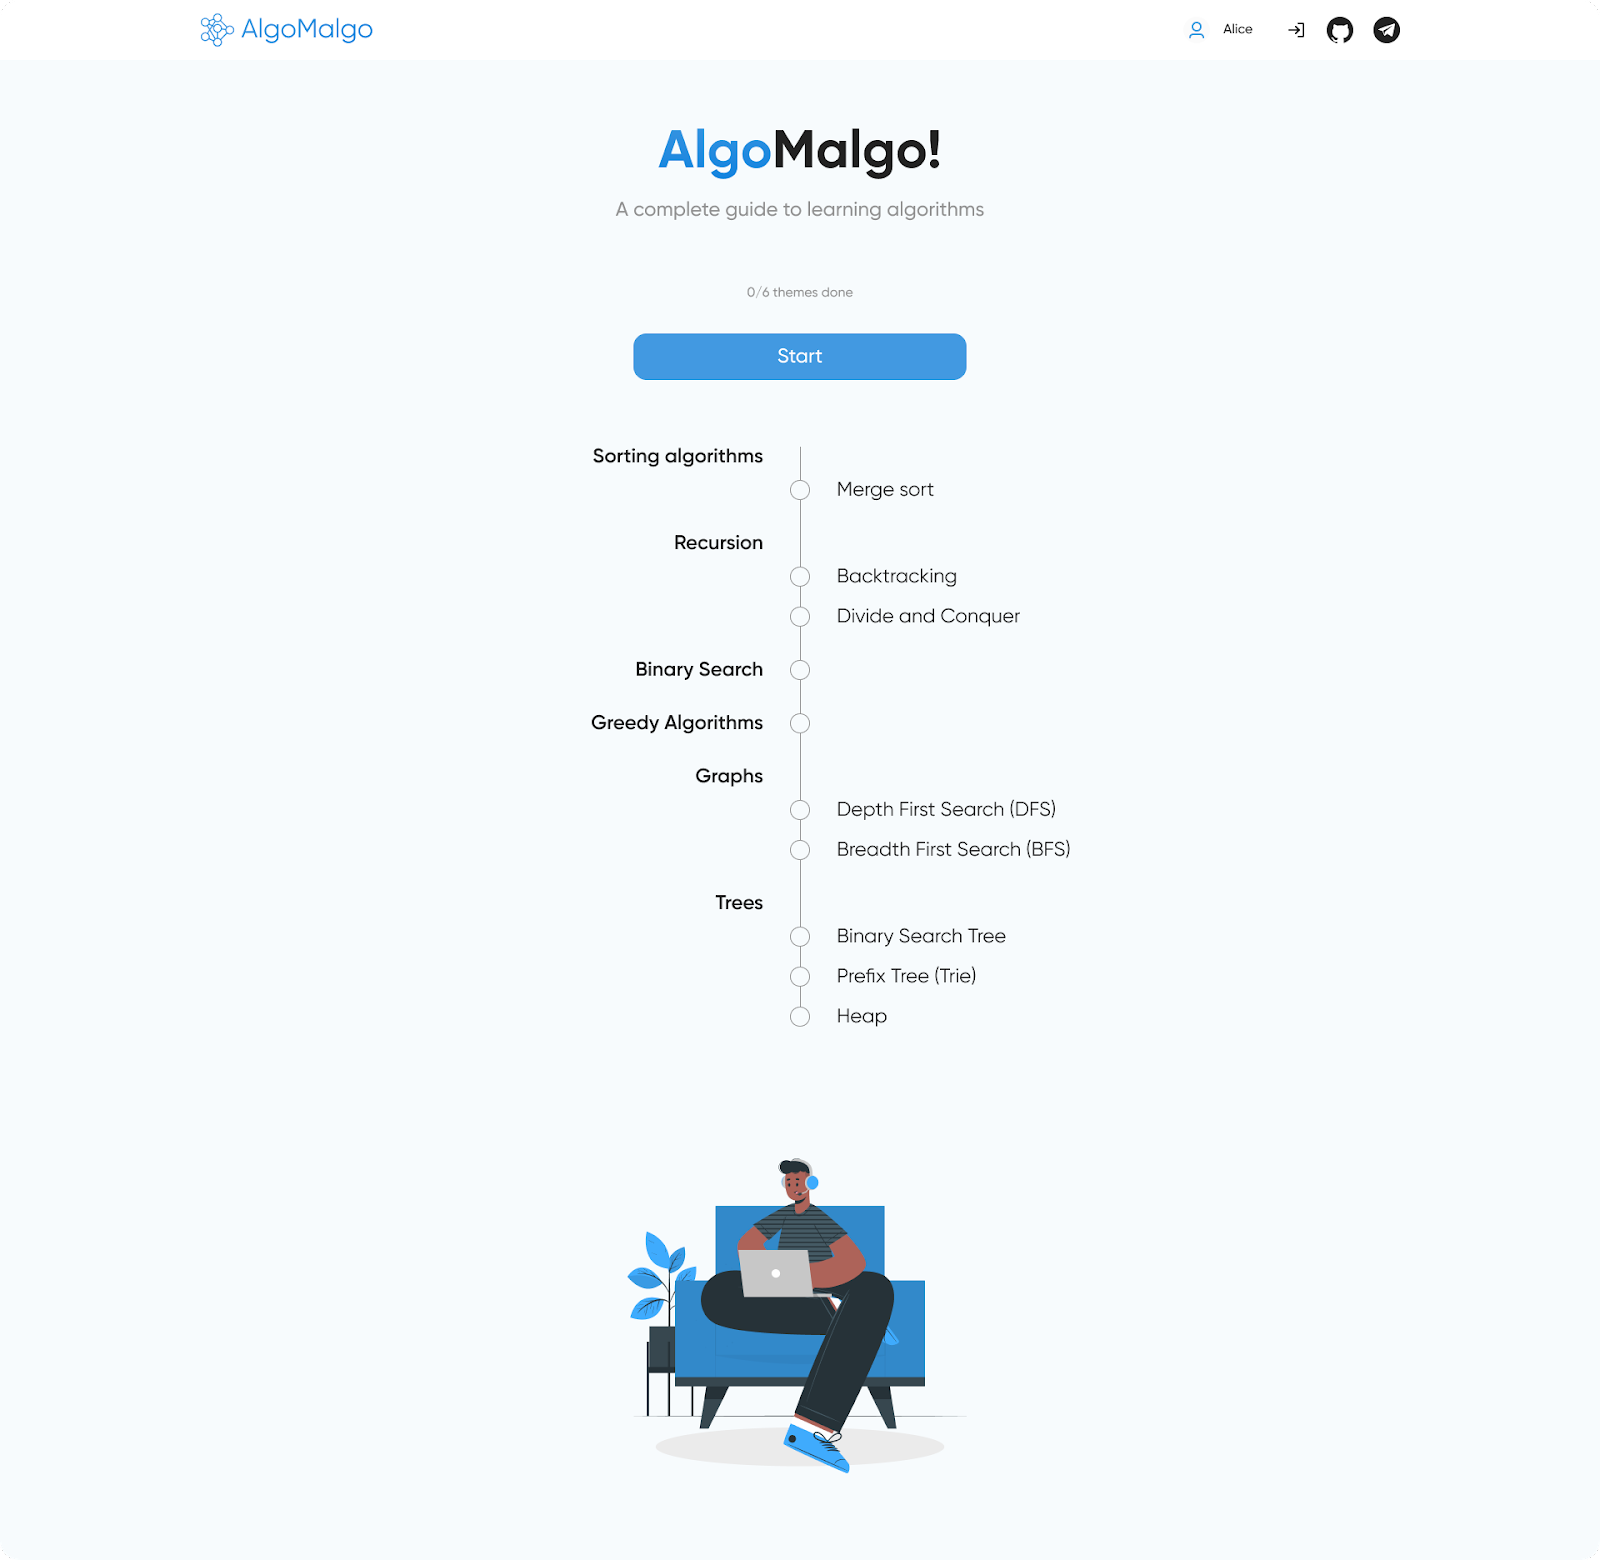
\includegraphics[scale=0.3]{figures/homepage.png}
    \caption{Home Page}
    \label{fig:gp}
\end{figure}


\pagebreak

\begin{figure}[h]
    \centering
    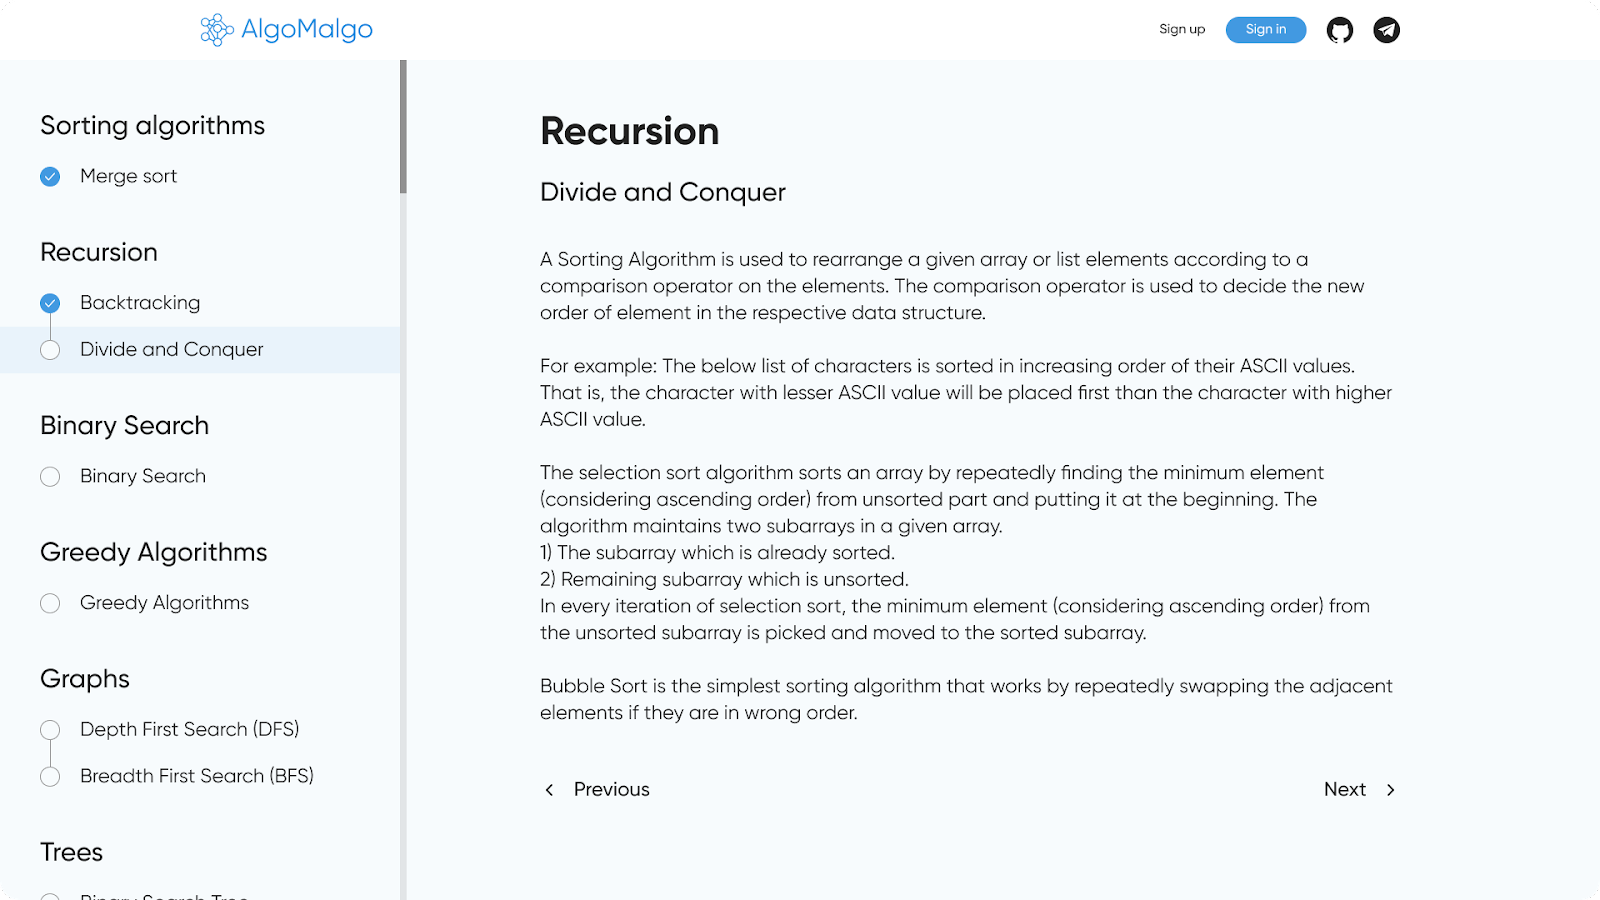
\includegraphics[scale=0.3]{figures/content.png}
    \caption{Content}
    \label{fig:gp}
\end{figure}


\pagebreak

\begin{figure}[h]
    \centering
    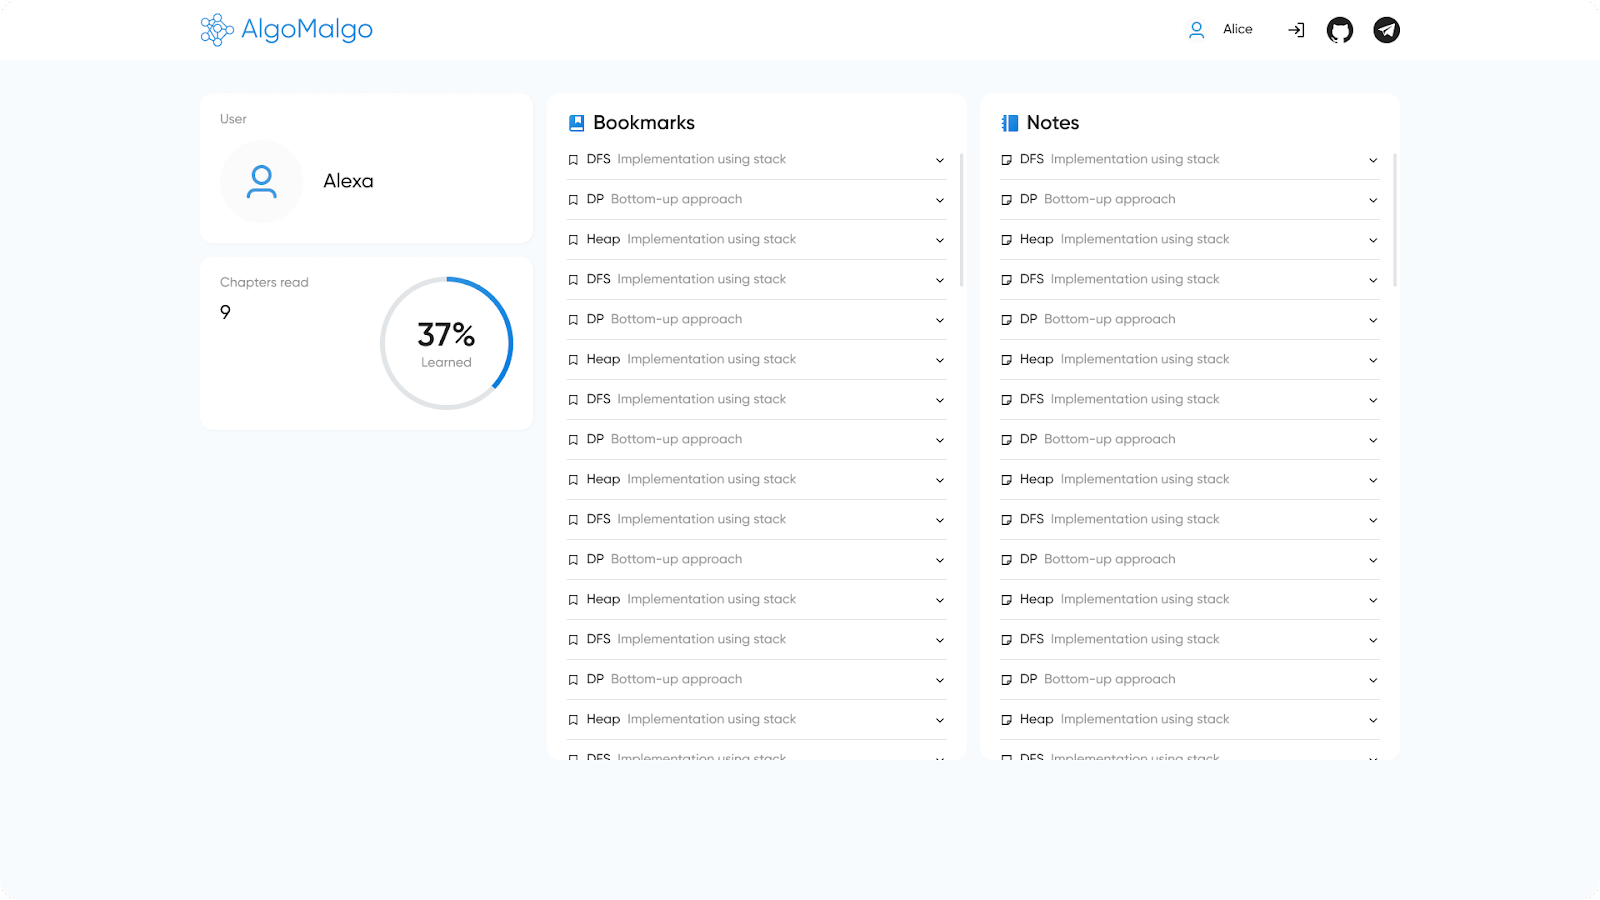
\includegraphics[scale=0.3]{figures/dashboard.png}
    \caption{Dashboard}
    \label{fig:gp}
\end{figure}


\pagebreak

\subsection{System Architecture}
System architecture of AlgoMalgo will be based on microservice, due its scalability and flexibility. Thus, with the increasing demand for our service, system design of website will change. As a main cloud computer provider AWS will be used, because of its cost-efficiency, flexibility and scalability.


\begin{figure}[h]
    \centering
    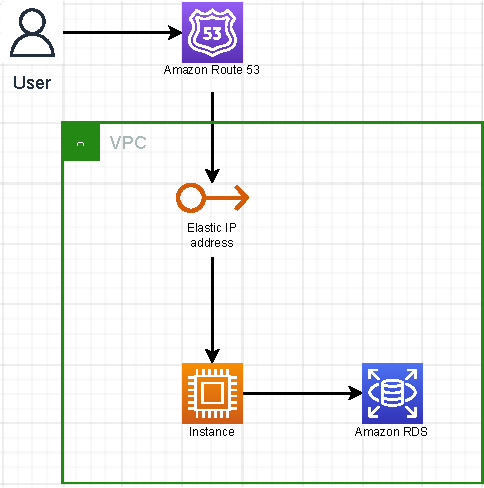
\includegraphics[scale=0.85]{figures/d1.pdf}
    \caption{100 users}
    \label{fig:gp}
\end{figure}


\pagebreak

In the above diagram, architecture is focused to embrace the number of users from 100 to 1000. As a main components Amazon Route 53, Elastic IP address, Instance and Amazon RDS will be used. All of them will be under virtual private cloud (VPC).

\begin{itemize}
  \item Amazon Route 53 component will be an extremely reliable and cost effective way to route end users to Internet applications by translating domain names to the ip address of our instances.
  \item Elastic IP address is used to mask the failure of an instance or software by instantly remapping the address to another instance in the user's AWS account.
  \item Instance is a server where app will be hosted
  \item Amazon RDS is a highly efficient solution for our relational database needs
\end{itemize}


\begin{figure}[h]
    \centering
    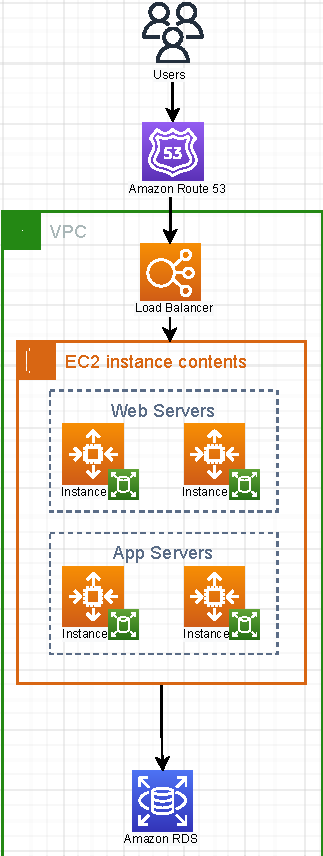
\includegraphics[scale=0.85]{figures/d2.pdf}
    \caption{1000 users}
    \label{fig:gp}
\end{figure}

\begin{itemize}
  \item EC2 instances will be used instead of simple instances, because of its auto-scaling capabilities. This feature will be helpful, in the situations, when the number of users will exceed the normal expectations. Thus, in days of extreme load, our application will remain healthy
  \item Elastic Block Stores is a green component attached to each EC2 instance in the above diagram. It serves as a cache block to each EC2 instance, so that service will remain fast.
  \item Load Balancer is a key component in every system that has more than 10000 users. This entity used to evenly distribute the load across existing EC2 instances to remain stability of the existing system.
\end{itemize}

To maintain the number of users from 1000 to 50000, Load Balancer, EC2 instances will be used. Furthemore, to evenly distribute the load, application logic and web logic will be hosted on different servers.

\begin{figure}[h]
    \centering
    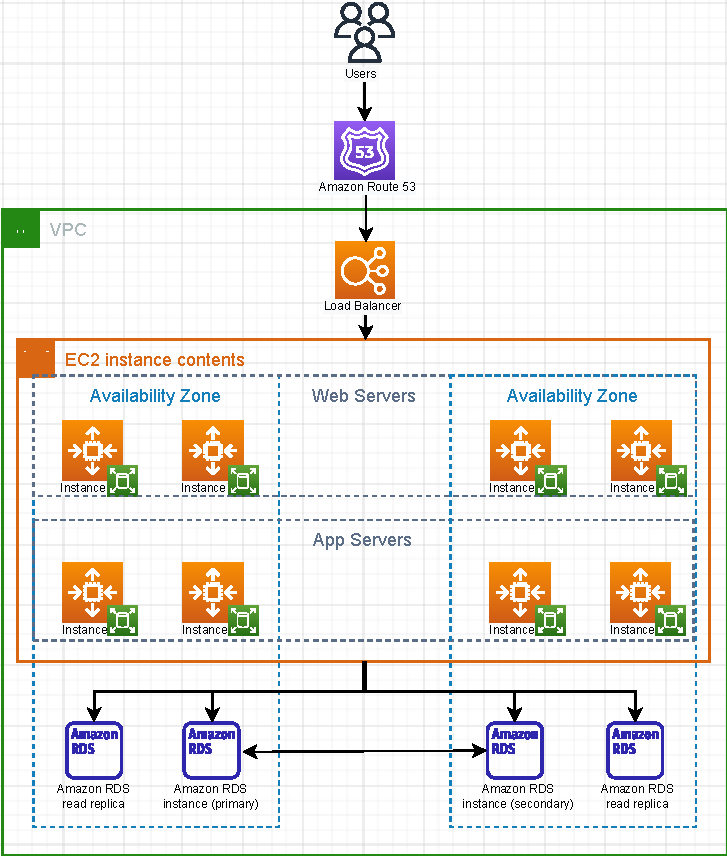
\includegraphics[scale=0.85]{figures/d3.pdf}
    \caption{1000 users}
    \label{fig:gp}
\end{figure}

Diagram above, indicates a good system architecture that could maintain the number of users from 50000 to 200000. Key components of the new system are RDS read replicas, RDS primary and secondary instances, and different availability zones.

\begin{itemize}
  \item RDS read replicas used to lower the load from RDS primary replicas, so that primary RDS replicas will handle only write requests. In the application it is supposed that the read operation requests will outperform by the number write requests. When the number of users will increase, the number of read replicas will increase proportionally.
  \item Availability Zone is a specific data point where EC2 instances and RDS components will be hosted. More Availability Zones indicate different data points, which will be located in different areas, so that users will not experience delays due their different locations across the country.
\end{itemize}


\begin{figure}[h]
    \centering
    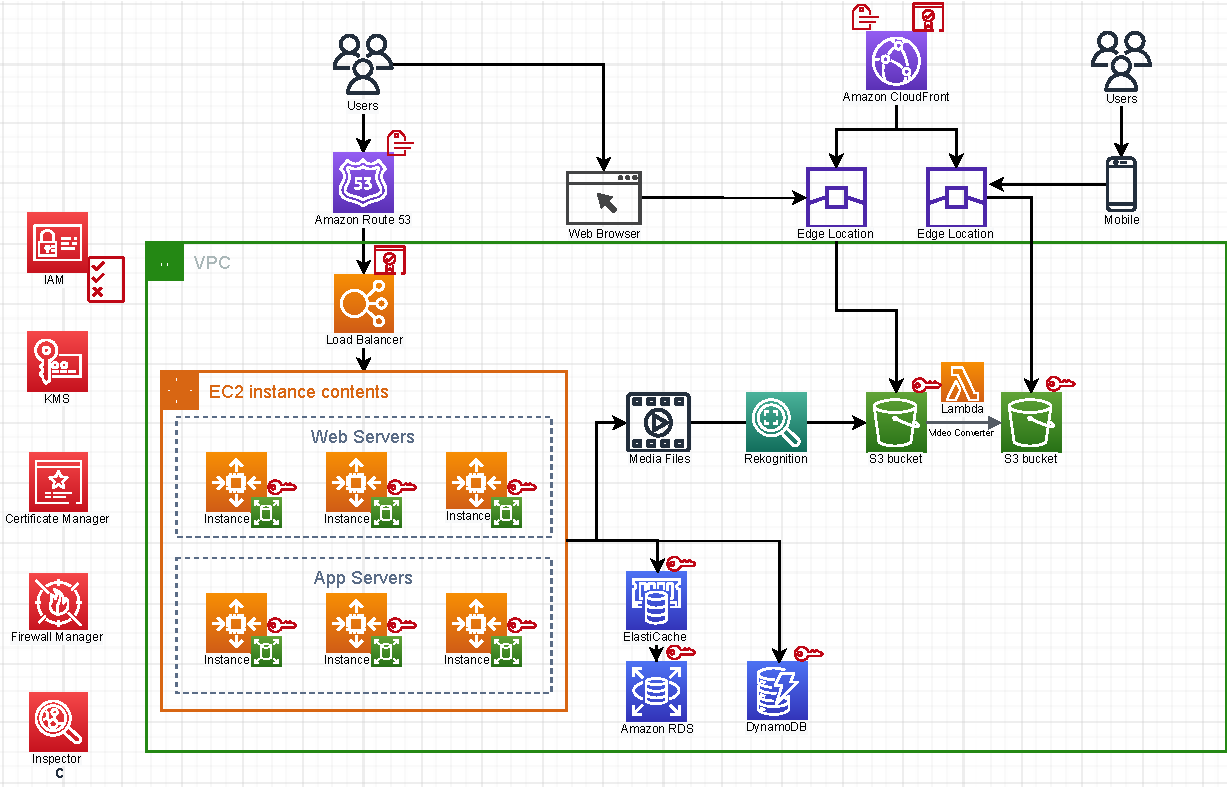
\includegraphics[scale=0.5]{figures/d4.pdf}
    \caption{10000 users}
    \label{fig:gp}
\end{figure}

System architecture shown above designed to support the number of users from 200000 to 1 million. There are many new components such as: IAM, KMS, Certificate Manager, Firewall Manager, Inspector, Rekognition, S3 buckets, Lambda, ElastiCache, DynamoDB, EdgeLocation and Amazon CloudFront. Services as IAM, KMS, Certificate Manager, Firewall Manager and Inspector responsible for security measures. They provide great security out of box, which will be essential for a service having around 1 million users. Different availability zones, Database read replicas not shown in this diagram to keep it clean. \\

\begin{itemize}
  \item Identity Access Manager is IAM in short. It is a primary service for managing all accesses of users in our AWS system. Accesses, authentication, authorization, restrictions managed by IAM. It will be used to give different permissions to a particular set of users, to manage an entire architecture.
  \item Key Management Service is KMS in short. It is a primary service responsible for all encryptions of data across the system. Services like DynamoDB, AmazonRDS, ElastiCache, S3 buckets and elastic block stores will be affected by KMS.
  \item Certificate Manager will be mainly responsible for providing SSL certificate to make secure HTTPS connections to services like Load balancer and Amazon CloudFront.
  \item Firewall Manager’s key responsibility is preventing different web site attacks including cross-site scripting, SQL injections, DDoS attacks, etc. This application firewall will secure such components as Amazon Route 53 and Amazon CloudFront.
  \item Inspector scans existing machines for the purpose of finding any known vulnerabilities, so that developers will fix them.
  \item Rekognition serves as a content filter, which will find out inappropriate objects in an image and will prevent this image being uploaded to S3 bucket.
  \item S3 bucket is an unlimited external storage, content on that storage could be accessible from any endpoint on the internet. In our system S3 bucket is mainly used for storing user media files, like images and videos.
  \item Lambda is a serverless service of Amazon, which will be used to convert one media format to another. It is expected that having 1 million users, that some of them will access AlgoMalgo through mobile phones. To maintain good user experience, it is essential to convert media files specifically for their devices.
  \item ElastiCache is a cache service for RDS databases. It comes with Redis and Memcached engines in it. Using ElastiCache we will reduce database calls, so that data that is accessed often will not heavily load RDS.
  \item DynamoDB is a NoSQL database solution. It will be essential for storing BookMarks and Notes logic. Currently, BookMarks and Notes stored in RDS, however having 1 million users it will be a wise decision to store these data on NoSQL database.
  \item Edge Location is a nearest location, where static content will be cached.
  \item CloudFront is a content delivery network (Cache), that is used for caching static content through accessing the nearest edge location. It is a good solution for caching any media content like images and videos. Because our system consists of detailed video explanations of algorithms and has various images explaining step by step solutions, it would be a great idea to have such service.
\end{itemize}

\chapter{Conclusion}\label{ch:concl}
The purpose of this thesis was to understand how promising and effective gamification in education is. Based on the amount of interest in this topic and successful applications in various fields, it can be assumed that gamification has good potential in the future. We examined the key elements of game elements that are successfully used in various fields of education. We analyzed the gaming industry and tried to find out the reason why so many people play different types of games.

\appendix
\input{appendixA}
\input{appendixB}
\printbibliography[heading=bibintoc,title={References}]

\end{document}
